\documentclass[12pt]{report}

\usepackage{url}
\usepackage[numbers,sort]{natbib}
\usepackage{graphicx}
\usepackage{amsmath}
\usepackage{amssymb}
\usepackage{algorithm}
\usepackage{algorithmic}
\usepackage{svg}

% If there are any other \usepackage commands, put them here.
\usepackage{amsthm}

\usepackage{lib/style/guthesis} % Must be the last package
\usepackage{hyperref}
\hypersetup{
  colorlinks   = true, %Colours links instead of ugly boxes
  urlcolor     = blue, %Colour for external hyperlinks
  linkcolor    = black, %Colour of internal links
  citecolor   = black %Colour of citations
}


\newtheorem{theorem}{Theorem}[section]
\newtheorem{question}{Research Question}
\newtheorem*{keyq}{Key Research Question}
\newtheorem{adversary}{Adversary Model}

% To comment out multiple lines of text.
\long\def\comment#1{}

\title{Peering Through Censorship:\\Tackling Internet Censorship Using P2P Networking}

\author{Eliana V. Troper}

\previousdegree{A.B.}

\thisdegree{Master of Science}  % or Doctor of Philosophy, etc.

\thisdiscipline{Computer Science}

\thesistype{Thesis}     % or Dissertation

% defense or approval date, not today's date...
\thesisday{11}
\thesismonth{April}
\thesisyear{2023}

\professor{Micah Sherr}

\fulltitle{Peering Through Censorship: Tackling Internet Censorship Using P2P Networking}

\indexwords{[TODO], Theses~(academic)}

\dean{Alexander Sens}

\memberi{Lisa Singh}
\memberii{Benjamin Ujcich}

\begin{document}

\pagenumbering{roman}

\maketitle    % Creates title page, copyright page if any, and approval page.

\begin{abstract}
TODO: Optional for master's thesis but these are nice (max 350 words)
\end{abstract}


\chapter*{Dedication}

TODO: Optional

\pseudochapter{Acknowledgments}

TODO

\tableofcontents

\listoffigures  % Optional - Omit this line if you don't want a list of figures.
\listoftables   % Optional - Omit this line if you don't want a list of tables.

\newpage

\pagenumbering{arabic}  % Ordinary pages have Arabic numerals.

\chapter{Introduction}

The internet has become a staple of the modern world, used by nearly every person on Earth.[CITE] The internet is a collection of independently managed networks which can route arbitrary traffic between said networks. It is built upon numerous \emph{protocols} which have been designed and iterated upon both academically and through practical usage over decades. Traffic on the internet travels from the edge of one network into another.\footnote{\emph{See} \ref{networking} for more on networking and key networking concepts.} This high level view loses some key context: networks are run by entities who have their own desires and are free to operate their network as they see fit. In an ideal world, all of these entities would run the same algorithms and would move traffic in a content-agnostic fashion, but we do not live in an ideal world. Various confounding factors result in a web that looks drastically different in practice from idealized theory: malicious entities use the web to perform attacks, bugs cause unforeseen issues to arise, entities want to tightly control traffic and content in their network, among other complicating factors.

The complicated, real internet leads to issues that do not arise in pure networking theory, one of which is \emph{censorship}. Censorship has become a loaded term in the current political context, and we do \emph{not} mean the colloquial usage of censorship. Censorship, as we discuss it, refers to entities censoring web traffic (either through complete blocking or other manipulation) at nodes (frequently routers) in the network(s) that they control. Censorship may be done for a variety of reasons - most censors claim they are solely removing malicious traffic, however, an entity may use their own definition of malicious which differs from colloquial usage of the term. We see some entities that choose to block social media sites, news sources, or any site that they deem block-worthy. Censors have a variety of justifications for their actions such as economic protectionism, removing unsavory content, blocking dangerous content, and maintaining law and order. We see this and ask our key research question:
\begin{keyq}
Can we circumvent censorship?
\end{keyq}
This is a very broad question - to be able to address it in a concrete and scientific manner we must refine it and break out more specific and actionable research questions. To circumvent censorship, we must address what censorship is:
\begin{question}
What do censorship systems look like?
\end{question}

We explore previous work to answer this question. In the real world, we frequently see adversaries perform basic censorship actions, such as blocking IPs and DNS resolutions. We also see adversaries taking more extreme actions, such as performing fingerprinting attacks or other techniques involving deep packet inspection (DPI).\footnote{\emph{See} \ref{real} for our exploration of real-world adversaries.} In theory, we see formulations that involve either attacking specific protocols [TODO e.g. xref Wang discussion] or employing a specific technique of attack applicable to several systems. [TODO: xref Salmon discussion] This allows us to refine our key question to focus on concrete systems:

\begin{keyq}
Can we circumvent censorship systems? If so, how?
\end{keyq}

As we discussed above, we note that some entity is performing censorship - censorship is not occurring spontaneously. Systems are not deployed magically, and do not arise without a concerted action undertaken by an entity. These systems are being designed and implemented by some entity to achieve a specific purpose. This leads us to our next research question:

\begin{question}
Can we define an adversary and model their censorship systems?
\end{question}

Previous work has spent significant time defining adversaries in order to posit new methods of circumvention, and we define our adversary in a similar fashion. Our adversary has unlimited resources, constrained only by physics and algorithmic limitations.\footnote{\emph{See} \ref{adversary} for our full definition and further discussion.} In our model, we also assume there is at least 1 location \emph{not} under the control of any censoring adversary.[XREF sphere of influence] Our theoretical adversary is informed by both real world observations and theories developed in prior work. In prior work, most adversarial models are highly focused - rather than looking at how an adversary may choose the full setup of a censorship suite, adversary modelling focuses on an adversary trying to tackle just one method of circumvention, and the broader picture is ignored. We formulate a model for evaluating an adversaries actions that looks at the \emph{whole} of their censorship apparatus:\footnote{\emph{See} \ref{theory} for more details and the derivation.}

\begin{equation}
[TODO: insert the final equation after cleaning notation]
\end{equation}

This model of an adversary is a novel contribution and allows for rooting research in the field to both the real world and existing theory. With an adversary and model defined, we can further refine the key research question tackled in this paper:

\begin{keyq}
Can we circumvent our adversary's censorship systems? If so, how?
\end{keyq}

We cannot immediately answer this question - as we see in our model, an adversary has some utility function. We start by bounding our potential utility functions with one of the [edge possibilites]: Consider a utility function where an adversary does not care about blocking access to sites they deem legitimate (i.e., blocking an allowed site has a utility to the adversary of $0$), but they feel strongly that no user should access a non-legitimate site (i.e. a user accessing a non-legitimate site has a utility of $-\infty$). This adversary would simply shut down \emph{all} traffic. This would provide them with $0$ utility, which is their maximal utility. In fact, in some instances censors have had real-world utility functions that result in actions like this, though those instances have been short lived.[CITE] However, in practice, we also see that no censor has continually provided 0 internet access - indicating that real world adversaries place a positive, non-zero value on allowing access to legitimate sites, even if they place a very negative value on some non-legitimate sites. While we can come up with infinite theoretical utility functions, we should focus on real and realistically possible utility functions, leading us to another research question:

\begin{question}
What does a realistic utility function look like for a censor?
\end{question}

We rely on looking at previous work focusing on real world adversaries to tackle this question, as well as novel contemporary observations. We find that most censors, in most circumstances, wish to censor users while providing access to acceptable sites. We also see that censors frequently fail to block some traffic that they could block using known methods. This brings us to the key concept of \emph{collateral damage}.[TODO: xref] A censor can employ censorship techniques to stop some traffic that they wish to stop, [but many methods of censorship would result in shutting down access to some allowed traffic]. We see several real world adversaries each employ unique censorship systems with varying degrees of collateral damage. [TODO: Add a bit more] As such, we refine our key research question:

\begin{keyq}
Can we circumvent our adversaries censorship system, given a realistic adversarial utility function? If so, how?
\end{keyq}

First, if we \emph{only} look at \emph{current} censorship apparatuses and real-world adversarial utility functions, we could conclude and say yes - based entirely on previous work. In practice, we see that the circumvention system Snowflake is currently working under all real-world adversaries. However, adversaries \emph{do} change their utility functions, and new censorship systems arise. Adversaries are trying to develop new systems, and so we cannot assume a system will function as well as it does currently indefinitely.\footnote{We note that a circumvention system which is provably able to survive could arise, however existing tools either do not have a strong scientific proof (e.g. Snowflake [XREF]) or proofs are frequently constrained to such an extent that they work in theory, but neglect an attack outside of the scope of that theory (e.g. Obfs and the bridge distribution problem [XREF]).} We look ahead to a potential adversary either adopting a different utility function with a higher tolerance for collateral damage or the development of a new censorship system that is more optimal than currently deployed systems. This leads us to our next research question:

\begin{question}
What might censorship look like in the near future?
\end{question}

We review related work and synthesize some possibilities for actions an adversary may take in the future. We focus on currently successful circumvention techniques, and provide some methods of censorship an adversary may engage in to further restrict these systems using existing techniques that might increase collateral damage. We also explore censorship techniques, and we observe that deep packet inspection and bridge enumeration are the two broad techniques an adversary may use in a more advanced censorship system. We discuss some directions that these techniques may proceed in. [TODO: More + be more concrete] We use this to refine our overarching research question into an approachable question:

\begin{question}
Can we circumvent our adversaries existing or potential censorship systems, given a realistic adversarial utility function? If so, how?
\end{question}

We address this by combining several observations which result from the answers to our previous questions:
\begin{itemize}
  \item A realistic censorship system should be based upon \emph{real} censorship systems and \emph{real} adversaries, with some further constraining beyond real-world adversaries allowed.
  \item Circumvention systems that thwart real censorship systems exist both in theory and the real world, but some functional systems \emph{primarily} exist in theory.
    \begin{itemize}
    \item There must be some limitation(s) to systems that only exist in theory.
    \item The practicality of real-world systems is crucial.
    \end{itemize}
  \item Circumvention systems function by combining a bootstrapping channel and a circumvention channel.
    \begin{itemize}
    \item We see that successful bootstrapping is generally done using a high value channel that has reasonable latency, but may have low bandwidth.
    \item We see that the circumvention channels that are used in the real world must have reasonable latency \emph{and} bandwidth.
    \end{itemize}
\end{itemize}
We build our system based upon the following principles derived from those observations:
\begin{itemize}
  \item A novel circumvention system should be functional.
    \begin{itemize}
    \item Functional means both not blocked, and having practical latency and bandwidth.
    \item The system must function both when bootstrapping and relaying traffic.
    \end{itemize}
  \item A novel circumvention system should improve upon an existing system in at least one of the following ways:
    \begin{itemize}
    \item Increase collateral damage\footnote{This also includes using a novel method of circumvention, though that is not required - a system may be iterative.}
    \item Scalability
    \item Usability
    \end{itemize}
  \item A novel circumvention system should not face the limitations that primarily theoretical systems face
\end{itemize}

We choose to build a system that iterates on the success of Snowflake. We do this by using the same type of channel (WebRTC) to relay our main traffic. We also use a bootstrapping channel in a similar fashion to Snowflake.\footnote{We use a stand-in in our demo system.} This is where the similarities end. We build our system as a standalone P2P system, which allows us to improve on Snowflake in several ways:

\begin{itemize}
  \item Increase collateral damage
    \begin{itemize}
    \item In existing systems, adversaries need to perform censorship solely at international gateways, but our system requires them to expand their censorship apparatus to cover intranational traffic as well. This drastically increases collateral damage, as adversaries have not been observed performing notable on-the-wire censorship within their borders. Adding intranational censorship will take any collateral damage that would have occurred solely to international endpoints and expands that to intranational end points as well.[TODO: mention/cite that most traffic is intranational]
    \item We use IPFS as a library for our channel, and any blocking of our system would result in blocking IPFS as well, blocking a protocol that is in use across the globe.
    \end{itemize}
  \item Scalability
    \begin{itemize}
    \item Snowflake is entirely volunteer run, and has encountered scalability issues in the real world in the last year as a result. There is some evidence that the volunteer base is largely saturated, and growing the network further is difficult. We address this by having every user of our network \emph{also} act as a provider of our network. This means that each node in our network does not solely drain system bandwidth, instead they use some bandwidth and also provide some bandwidth.\footnote{A user may provide more bandwidth than they use, however, an exploration of the bandwidth provided vs the bandwidth used of users of our network would require numerous real users.}
    \end{itemize}
  \item Usability
    \begin{itemize}
    \item We build our system as a standalone system, allowing users to use our system without the reduction of usability that comes with using Tor.\footnote{We emphasize that users could potentially use our system to access Tor, but they are not required to, increasing usability in instances where a user does not need anonymity.}
    \item Our system can be transferred and run as a singular HTML file in any relatively up to date web browser.
    \end{itemize}
\end{itemize}
[END TODO: If any of these remain single bullet points, switch to `ITEM: TEXT` instead of nested lists]

In practical terms, we build a system by using LibP2P and IPFS as libraries, and building a dynamically updating tree which contains metadata and pointers to hashes of files - which can then be retrieved over IPFS. We also outline some attacks a censor may take against IPFS, and we modify our usage of IPFS to mitigate these attacks. We build both Golang and Javascript libraries which are used to access and update the aformentioned tree, as well as to establish uplink channels. We build a benchmarking app on top of our network, as well as some demo apps [TODO: list final apps].

We then use our benchmarking app to demonstrate how our system works in a variety of conditions, based upon some of the potential actions a censor may take:
\begin{itemize}
  \item No censorship
  \item Censoring fixed nodes
  \item Censoring fixed nodes \emph{and} all traffic except WebRTC and email.
\end{itemize}

The second test is in line with how adversaries currently function in the real world, and the third test posits an adversary which has a utility function more extreme than existing adversaries. We note that we do not spend extensive time looking at DPI attacks on WebRTC - this is because these are generally fingerprinting attacks, and because we use the built in WebRTC from standard web browsers, there should not be any fingerprint distinct from standard usage of WebRTC.\footnote{An adversary may perform \emph{content} fingerprinting attacks, however, we relegate these attacks to future work, and note that adversaries do not appear to do these in practice in the realm of censorship, and they have false positive rates too high for usage. [CITE] [XREF false positives]}

[TODO: Explore speed results]

We then conclude and offer a discussion on ethics of our system and potential future work.[XREF]

[END TODO: Check paragraph indentation]
[END TODO: Add xrefs throughout]
[END TODO: Add cites throughout]

\chapter{Background}

The term censorship has taken on a life of it's own in the modern social and political context. We are \emph{not} exploring the general connotation of censorship, rather, we are exploring a specific type of censorship that existing in a networking (particularly inter-networking) context. We will explore some key concepts and present a short model of networking.

\section{Networking concepts}
\label{networking}

We are going to consider the internet as it currently exists, rather than historical states of the internet. Some key concepts:

\begin{itemize}
  \item Internet Protocol (IP) addresses: These are used to represent endpoints of a connection, and are used for routing. Within a network, other identifiers, such as MAC addresses, are used for routing, however, we are focused on routing between networks and will only consider IP based routing as we explore censorship circumvention. We will use IPv4 addresses throughout as sample addresses, though conceptually IPv6 addresses function similarly for the focuses of this paper.
  \item Domain Name System (DNS): DNS resolution is used to map from human-readable and memorable addresses that map to IP addresses (e.g. georgetown.edu resolved to 23.185.0.2 at the time of writing). [TODO: Explore the transparency of these, DNSSEC, etc]
  \item Router: Routers perform routing for networking, as well as other functions that act on network traffic. They may be the home of a NAT, a firewall, or censorship software. The controller of a router may access and manipulate any traffic which passes through it.
  \item Firewalls: These are software that may restrict traffic based on rules. These rules may be simple or complex. These have positive uses, such as securing a network from attacks.
  \item Network address translation (NAT): A NAT is used to map network addresses seen on one side of a router to those seen on the other side of a router. These are frequently used to house potentially thousands of devices behind a single internet facing IP address. Most humans use devices located behind a NAT.
\end{itemize}

\begin{figure}
\begin{center}
{\includesvg{figures/networking}}
\end{center}
\caption[Basic networking]{A model of networking, sufficient for exploring censorship circumvention [TODO: Add final arrows, some sample traffic]}
\end{figure}

\section{What is censorship circumvention?}
\label{circumvention}

When we discuss the subfield of censorship circumvention when discussing networking and security, we are \emph{not} discussing all forms of censorship that a web user might face - we are discussing censorship on-the-wire of active internet traffic, which usually consists of blocking access to specific services. We do not consider a service blocking certain conduct (e.g. a social network restricting hate speech) the censorship that we are circumventing. We aim to allow a use to connect to any service they would like (notwithstanding technical limitations) - not to allow a user to use any service how they would like. Throughout this paper, when we mention censorship, we mean on-the-wire censorship of reaching services.

\subsection{Ethics}

We recognize that some users run heinous services on the web - most of which are illegal in any existing jurisdiction. We believe that the best approach for ceasing access to these heinous services is best done through a legal system - IE, investigating and identifying the perpetrator(s), turning off the service directly, and prosecuting any perpetrator(s) of said acts. We note that most morally reprehensible acts that are frequently associated with anonymity and censorship circumvention systems involve actions that occur in the real world (e.g. exploitation of children, weapon/drug/human trafficking all involve actions that occur in the real world either prior to distribution on the internet or triggered by actions on the internet).

The only notable class of crime which can occur without physical, real-world actions is piracy/IP violations. We believe that targeted legal actions (e.g. DMCA take-downs) can mitigate the issue, and that the cost of further mitigation through censorship would lead to large collateral damage of legal content and a chilling effect of legal speech and usage of the web, and as such the possibility of a circumvention system being used for piracy/IP violations is an acceptable risk given the ability to mitigate damage through the legal system.

\subsection{Threat model and adversary}
\label{adversary}

Censorship circumvention is an abstract concept, and approaching it in a scientific way requires properly defining and scoping the task. We have already defined the task, [TODO: xref] and must now scope the problem. We will scope our problem by creating a \textbf{threat model} of the censor we are aiming to thwart, termed \textbf{the adversary}.

An adversary has an \textbf{area of influence}. This is an area an adversary controls the network of, and can control (either directly or through compulsion) any service providers within. We assume an adversary may have an area of influence consisting of several nations, with at least one nation outside of the area of influence of \emph{any} censor.\footnote{This does not mean that this nation does not have the technical capability to censor, but rather does not perform any censorship either directly or via threatening a start of censorship.}

Our adversary has effectively infinite resources, but is bound by the laws of physics and as such is bounded by the difficulty of computational problems (and the known solutions to these problems, e.g. even if P=NP, the solution is not known, and as such cannot be used). These resources may include labor, capital, technical expertise, and total control of the legal system.

We also assume that our adversary has access to the source code of any circumvention system available, and knowledge of the existence of our circumvention system. We discuss why security through obscurity cannot be used in an effective circumvention system in [TODO: xref].

We also assume that our adversary only takes actions \textbf{on-the-wire} and at \textbf{service providers} within their area of influence - effectively, the adversary isn't interested in any individual in particular and is performing a dragnet operation, rather than an operation targeting a specific entity. We can use a thought experiment to justify this: if an adversary had a person looking over your shoulder or using video surveillance, they could simply look at what you are doing and punish you directly, no need to expend the resources needed to censor the web.

We assume our adversary has some interest in the utility of the internet and certain technologies on the internet. This means two things: an adversary will not shut down the internet in it's entirety\footnote{Internet shutdowns are a trivial way to censor forbidden internet usage - at the expense of shutting down any non-forbidden usage. [TODO: Discuss prior shut downs in another section and xref]} and an adversary has some threshold of unacceptable collateral damage caused by potential censorship techniques.\footnote{Similar to a full internet shutdown, if an adversary wanted to block all access to a specific HTTP site, they could block \emph{all} HTTP traffic, at the expense of blocking every HTTP site. This piecemeal web censorship could even be thwarted with a circumvention system that simply proxies HTTP traffic outside of the area of influence within an unblocked protocol and connects to HTTP sites from outside the area of influence. This starts to show that any non-complete shutdown of internet traffic may have gaps for circumvention techniques. We discuss collateral damage further in [TODO: xref].}

Finally, we note that any technique that subverts this adversary will also work when weakening the strength of these assumptions - e.g. if the adversary controls one nation instead of several, we have more area to run a circumvention system from; if the adversary is only willing to take actions at service providers and not on-the-wire, anything that can thwart an adversary that takes both actions could trivially thwart the adversary that only performs actions at one. We also note that a system could detect the type of actions an adversary is taking and maximize performance based upon what subset of possible actions an adversary is taking - e.g. an adversary that is not touching services leaves an easy path for a circumvention system to use - those services themself.

[TODO: Basic model + adversary]

\begin{figure}
\begin{center}
{\includesvg{figures/networking}}
\end{center}
\caption[Basic networking, with an adversary]{A model of networking, with our adversary model overlaid [TODO: Once networking diagram is finalized, add an adversary]}
\end{figure}

\subsection{User model}

[TODO]

[TODO: We should outline that we do not assume unlimited resources for our system. We should outline that we expect users to run the software on a phone or basic computer, and that we expect the system to be run by volunteers (who may or may not have significant resource)]

\subsection{System provider model}

[TODO]

\subsection{History and basics}

The web arose in a relatively haphazard fashion [TODO: discuss a bit more]. The web was not a place where adversaries engaged in censorship (if they paid any mind to the web whatsoever). Instead, as the web became more prominent and more global, individuals realized that they could be tracked, and that they desired anonymity. This led to the development of basic and advanced anonymity software, with proxying being a basic tool for this and Tor being the most prominent example of full fledged anonymity software.

As this occurred, the web continued to grow in prominence, and the concept of "Web 2.0" arose - regular users could post content to sites such as message boards and social media sites. People could organize quickly and effectively across larger distances and with people they had never met in the past. Governments took notice - and censorship began.\footnote{The main justifications censors employ are maintaining law and order, preventing the spread of disinformation, preventing access to "unwholesome" content, or economic protectionism. [TODO: Would be cool to cite one or several instances of these justifications coming from the horses mouth]}

When internet censorship arose, basic techniques were used. These include:
\begin{itemize}
  \item Blocking specific IPs: Traffic to or from various IP addresses could be dropped. This is simple and low cost.
  \item Blocking DNS resolution: DNS resolution traffic for specific requests could be dropped (or replaced). This is simple and low cost. [TODO: address DNS encryption and authentication]
  \item Legal mechanisms: If a service exists within the area an adversary controls, they could simply take down the service itself. Since we define the adversary to not control the whole world, we will ignore this form of censorship throughout this paper, as a restricted service could avoid this by relocating out of the sphere of influence of an adversary.
\end{itemize}
These techniques are sufficient to cut off access to services for users who are either unaware of a censor, unaware that circumvention is possible, users who do not care about the actions of a censor, or out of laziness. A user would have to actively use something that circumvents these simple blocks. The solution to avoid IP blocking and censoring DNS results is to proxy a users raw traffic outside of a censored area (either through a basic proxy, or something that provides other features, such as Tor). From the view of a censor, a user would not be accessing a restricted service, they would be accessing a proxy service.

\begin{figure}
\begin{center}
{\includesvg{figures/networking}}
\end{center}
\caption[Basic networking, with an adversary performing censorship]{A model of networking, with our adversary performing basic censorship [TODO: Once networking diagram is finalized, show blocking]}
\end{figure}

Censorship circumvention arose as a by-product of tools made for purposes that were not focused on censorship circumvention. As primitive censorship began, people realized that anonymity software such as Tor or even a basic proxy could be used to access services that would otherwise be blocked. The entrances to these proxy services and Tor were accessed via well known IP addresses or DNS names.\footnote{The reason these were well known is that, if you want the public to access your service, they must know how to access these services, including the addresses of your service. These must be made public to allow people to access your service. A censor has access to public information.} Censors began being blocking access to these services, in addition to their original censorship targets. This set off a "censorship arms race."

At this point, those who used and built the anonymity software recognized that censorship circumvention would be crucial for maintaining access to these tools, and others realized that censorship circumvention in-and-of itself would be useful. This effectively led to the rise of a subdiscipline that draws heavily from networking, security, and even game theory, but also exists independently from those subdisciplines, with a variety of stakeholders including governments, NGOs, non-profits, independent programmers, academics, and others interested in developing censorship circumvention techniques. This also leads to a relatively unique feature of this discipline - some techniques were developed in academia, some techniques were developed in the real world, and some were developed in both, and ignoring the results from either thread of research and observation can lead to the development of flawed systems.

\subsection{Current theory of censorship circumvention}

[TODO: Maybe cut? Or just point to next section]

The bedrock of the theory underlying successful provision of access to proxies is collateral damage.

[TODO: Discuss collateral damage more]

\chapter{Related Work}

Censorship circumvention has developped over several decades. Originating out of anonymity research, censorship resistance is a less difficult problem than full anonymity,\footnote{Anonymity generally requires censorship resistance (or a non-censoring adversary) to bootstrap.} and has become a topic studied on it's own independent of anonymity.\footnote{Though anonymity and censorship are distinct problems and are often approached independently in research, there is notable interaction between the two fields - many censorship circumvention techniques target the pluggable transport (PT) spec for deployment of censorship systems. The original PT spec was made for Tor, an anonymity network and protocol,\cite{tor} though later iterations of the spec are more general and are in use by tools including Tor, Lantern, and Psiphon.\cite{pt} In practice, current functional real world techniques all use the PT spec - see \ref{obfs} and \ref{snowflake} for details.} Censorship circumvention generally looks at one of two problems: proxying traffic \emph{out} of an adversaries sphere of influence, and providing access to those proxies to those within an adversaries sphere of influence.

[TODO: Add in new paper re: obfs]

\section{Prior proxying theory and techniques}

Most proxying techniques fall into one of three broad categories: looking like an unknown protocol, mimicing an existing protocol, or using an existing protocol as intended. Of these, mimicry was eliminated as a functional technique. Houmansadr et al established requirements that a mimicry system must meet to succeed - the imitated protocol must be mimiced in full, the imitation protocol must react properly to errors and network conditions, the imitation protocol must have traffic typical of the imitated protocol, and the imitation protocol must imitate artifacts from implementations of the imitated protocol properly.\cite{parrot} They continued by showing that none of the cutting edge mimicry protocols of the time were able to fulfill these requirements.\footnote{The authors explore SkypeMorph, StegoTorus, and CensorSpoofer - they quickly find passive attacks for these transports.\cite{skypemorph}\cite{stegotorus}\cite{censorspoofer}\cite{parrot}} The authors finally show that even with the initial attacks they find, hypothetical, improved transports that patch those would still fail as there are attacks that could not be prevented when imitating a proprietary protocol. The authors have a damning conclusion that has held until today: "unobservability by imitation is a fundamentally flawed approach, unlikely to ever suceed due to the daunting list of reqirements that an imitator must satisfy. The failure of all proposed [imitation] circumvention systems to achiever unobservability confirms this conclusion."\cite{parrot}

[TODO: Break down into high bandwidth/low bandwidth]

[TODO: For each of these be sure to mention if they work IRL]

TODO

[TODO: Do mention some things like shadowsocks that are in use but are even further from academics]

[TODO: Discuss fingerprinting, including contemporary examples w/ snowflake]

\subsection{Unknown Protocols}

TODO

\subsubsection{OBFS and Scramblesuit}

TODO

[TODO: Others]

\subsection{[P2P and P2P-like]}

TODO

\subsubsection{Snowflake}

TODO

[TODO: Add a diagram which will be used later to start to show "modifications" from the snowflake model to get our system]

[TODO: Iran case study to highlight scalability]

\subsubsection{MassBrowser}

TODO

\subsection{High-reliability channels}

[TODO: Mention stego]

TODO

\subsubsection{Domain fronting}

TODO

\subsubsection{Email}

[TODO: Mention this w/ raven, bridgedb, etc]

\subsection{Decoy routing}

TODO

\subsubsection{Tapdance}

\subsection{Tunneling and realistic behavior}

\subsubsection{Raven}

\section{Real world observations}
\label{real}

[TODO - a bunch of case studies]

[Important to hit: recent OBFS entropy attack, Iran study that shows slowdown, China, DNS/IP censorship, DNSSEC failure]

\subsection{Real world and academic theory}

[TODO - may cut this, but this will be drawing conclusions from our examples above, and comparing those adversaries to the adversary model we outlined, and will transition our discussion to OBFS/the bridge distribution problem]

\subsection{The bridge distribution problem}

[TODO - Salmon + that followup paper]

\section{P2P networking}

TODO

[TODO: Torrents, Crypto, ???]

\subsection{IPFS}

TODO

\chapter{Theory}
\label{theory}

We begin with a basic model - an adversary will engage in the censorship of service $x$ if $B_x - C_x > 0$, where $B_x$ is the average benefit per user of engaging in censorship of service $x$ and $C_x$ is the average cost of engaging in censorship of service $x$. We will refine this formula by switching to a focus on censorship techniques - $(b_{x,1} + b_{x,2} + ... + b_{x,n}) - C_x > 0$, where $b_{x,n}$ is the average benefit per user of censoring service $n$ using method $x$. A censor will engage in any censorship method where the average benefit reaped by censoring \emph{any} desired services using that method is greater than the cost. Also note that these benefits and costs are based on how they are \emph{perceived} by the censor, not by an objective, bird-eye view of good and bad, and they may account for a variety of benefits/cost, including direct financial costs, but also including less tangible value such as "stability".

We now note that each method may only stop a fraction of users accessing a service using a method - so a more realistic formulation would be $(u_{x,1}*b_{x,1} + u_{x,2}*b_{x,2} + ... + u_{x,n}*b_{x,n}) - C_x > 0$, where $u_{x,n}$ is the fraction of users accessing service $n$ that are blocked from accessing service $n$ using method $x$.

We will now break down cost further. $C_x = f_x + m_x$ - where $f_x$ is the fixed cost per user of setting up method $x$ and $m_x$ is the marginal cost of actively engaging in $x$ per user. We will drop $f_x$ from further consideration (IE, $C_x = m_x$) - the cost of setting up a method is a one time cost, and to an adversary with unlimited resources, expending a one time cost averages to $0$ over the long run. We will now explore the marginal cost of $x$. Censorship tools may slow down "good" traffic, and they may erroneously block access to good services. Therefore, $C_x = s_x*i_x + (u_{x,1}*c_{x,1} + u_{x,2}*c_{x,2} + ...  + u_{x,n}*c_{x,n})$, where $c_{x,n}$ is the average cost of blocking service $n$ per user, $u_{x,n}$ is the same as above, $s_x$ is the average fraction of the total value of unblocked traffic retained (due to the reduction in speed caused by enabling method $x$),\footnote{Note that an adversary may engage in multiple stages of filtering, so some subsets of unblocked traffic may experience no slowdown, while some might experience more. For the purposes of our analysis, we can use the average across all allowed traffic.}, and $i_x$ is the value per user of access to all unblocked sites. Combining the above, we see
$(u_{x,1}*b_{x,1} + u_{x,1}*b_{x,2} + ... + u_{x,n}*b_{x,n}) - s_x*i_x + (c_{x,1} + c_{x,2} + ...  + c_{x,n}) > 0$, or, more succinctly:
\begin{equation}
-s_x*i_x + \sum_{s=1}^{n}u_{x,s}*v_{x,s} > 0
\end{equation}
where $v_{x,s} = b_{x,s} - c_{x,s}$.

We could conclude here if a censor engaged in censorship solely using a singular method of censorship - however, censors engage in multiple methods of censorship, and the benefit of successfully blocking a site is not distributed multiple times if it's blocked by multiple methods, the benefit is only achieved based on new users blocked by a method, or, in short, a singular censorship system $x$ will be implemented if:
\begin{equation}
-s_x*i_x + \sum_{s=1}^{n}\Delta u_{x,s}*v_{x,s} > 0
\end{equation}
Note that all variables are the same, except $i_x$ is now the value per user of access to all unblocked sites prior to enabling censorship system $x$ and $\Delta u_{x,s}$ is the change in the fraction of users who can access service $s$ after enabling $x$.

We have now established an equation used to determine if a censor will enable an individual system, taking existing systems (or lack thereof) as a given. This is not reflective of reality, where a rational censor will evaluate \emph{all} of their active and potential circumvention systems in conjunction.

The valuation of a system consisting of censorship systems $1$ through $m$ is as follows:
\begin{equation}
\sum_{x=1}^{m}\sum_{s=1}^{n}\Delta u_{x,s}*v_{x,s} - i_{x} * \prod_{x=1}^{m}s_x
\end{equation}
All variables are the same as previously, except $i_x$ is the value per user of access to all unblocked sites again, $s_x$ is the average fraction of the total value of unblocked traffic retained after enabling all systems $y$ with $0\leq y<x$, and $\Delta  u_{x,s}$ change in fraction of all users blocked using method $x$ that were not already blocked after enabling all systems $y$ with $0\leq y<x$. We will define $x=0$ such that this "censorship" system is the null (non-existent) censorship system, and therefore $s_0 = 1$, and $u_{0,s} = 0$.

We assert that a censor is picking from a number of censorship systems that is small enough such that the censor can evaluate the above equation for every possible set of censorship systems in every permutation such that each set only has one of each censorship system in a reasonable amount of time. [TODO: Maybe justify a bit more?]

A rational censor will enable the set of censorship systems such that the above equation is maximized given every potential set of circumvention systems.

[TODO: Dig into the base rate fallacy, and expound on that with an equation based expansion that fits in the above model]

[TODO: Walk through one example using this]

\chapter{System design}

We saw that several circumvention systems work given the constraints they were designed for, however, these constraints are either too loose and have known real-world failures under our adversary model,\footnote{The bridge distribution problem being the most notable issue for several otherwise effective systems.} the systems are difficult to deploy, or they have scalability issues.

Additionally, usability is also a crucial issue [TODO: COVER THIS IN RELATED WORK], and we identify two crucial issues where at least one of these affects every previously discussed system:
\begin{itemize}
  \item Low bandwidth/poor performance: Users want a good experience on the web. Some of these methods are completely unusable for proxying the entirety of a web session. Additionally, many of these items are tied to usage of Tor. While we support usage of Tor, it slows down web browsing even without circumvention tools in use, and usage can [result in broken behavior on some websites/some sites block Tor TODO: explore and cite either in fn or related work].
  \item Barriers to entry: Every system we've explored that are usable by a layperson require usage in conjunction with Tor - and a layperson must be aware Tor exists, not be biased against it,\footnote{Some individuals believe that Tor is only used by criminals, and while we do not believe this is true, dispelling misinformation at a large scale is a herculean task that we will assume is not possible in the short and medium term [TODO: Citing this would be good]} know how to get it, and not be censored when getting it.\footnote{Acquiring Tor is frequently censored for users, which means that a user \emph{must} acquire it prior to being under a censorship regime, or must have some out of band channel for acquisition. [TODO: Worth citing, may be worth bumping up importance]}
\end{itemize}

Below, we propose a system with a clear theoretical backing and achievable goals based on both theory and real-world observations. [TODO: xref] We also address these other key issues.

\section{Theory and goals}

First, we want to define system goal and highlight some non-goals that are close to censorship circumvention, but are not directly used for them.

We aim to thwart the adversary we outline in [TODO: xref]. We will rely heavily on the concept of collateral damage. [TODO: xref]

We are \emph{not} aiming to provide anonymity.\footnote{Perhaps our system could be used to access an anonymity system, but we do not want to guarantee anonymity or guarantee that the system will not leak information that may break anonymity, though we are not deliberately trying to break anonymity, we are also not evaluating our system for it at this point.} We feel the need to emphasize this, as most current systems that are functional in the real world are used purely as a PT by Tor.\footnote{Our system could be used as a PT, as we do have a Golang implementation, however, evaluating this system for usage as a PT is reserved for future work. [TODO: XREF PTs]}

We will break down our goals into two sets: accomplishing censorship circumvention, and providing a more usable system for a layperson.

\subsection{Censorship circumvention}

Earlier, [TODO: xref] we discussed a variety of censorship circumvention systems. Observing how and why each of these work, and the drawbacks associated with each of them will allow us to formulate goals we wish to achieve, working techniques we may use, and a theory for our systems function. We present a short summary of previous systems in [TODO: xref table], comparing and contrasting their successful techniques and transports, and their individual drawbacks.

\begin{table}
\caption{Comparison of existing systems.}
\begin{center}
[TODO: Make table take whole page sideways, make in latex when finalized]
\makebox[\textwidth]{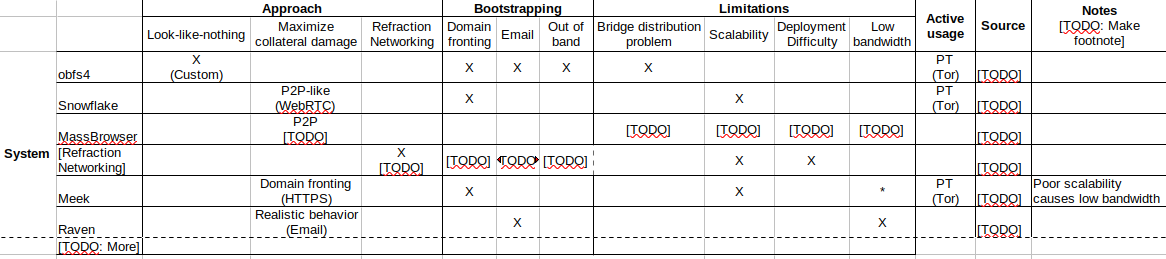
\includegraphics[width=\paperwidth]{tables/comparison-draft.png}}
\end{center}
\end{table}

We see that existing systems are limited by at least one of the following:
\begin{itemize}
  \item The bridge distribution problem [TODO: Xref]
  \item Scalability
  \item Deployment difficulty
  \item Low bandwidth
\end{itemize}

Another key observation is that \emph{collateral damage} is the bedrock of the theory behind \emph{all} circumvention systems - as such, any system must be based around maximizing this - the ideal system will make the only feasible way to shut down the system effectively shutting down a large portion of internet traffic. 

[TODO: Discuss false positives + the overhead of blocking traffic]

[TODO: More]

We first note that systems with deployment difficulty (refraction networking) as their primary limitation rely on either a single or handful of \emph{large}, \emph{continuously cooperative} entities (all very large tech corporations). This makes the circumvention method brittle - IE, a change of heart of very few entities could negate the effectiveness of this method. We believe that not only is this a possibility, but it is a \emph{likely} possibility - we note that adversaries may be as large as a collective of nations in our model - and given the profit maximization of corporations, these entities will want to perform business in the sphere of influence of our adversary. The adversary could pressure the entity to shut down the system in order to perform business within, with, and with citizens of the sphere of influence of the adversary. Economic theory implies that this will occur in the long run. [TODO: shore this up with both more clear wording and with some cites to examples] Due to this limitation we will not be building on refraction networking for our system.

[TODO: We will not use systems with the bridge distribution problem as their flaw, xref salmon section]

We are now effectively left with techniques with scalability and low bandwidth as our primary limitations to consider. Systems with low bandwidth are either directly limited through maximum channel bandwidth,\footnote{Even without system overheads - e.g. Raven reduces bandwidth from an already low level to an even \emph{lower} level.} or through financial cost. Because of our system and user model, where the system is run with potentially limited resources and users are not charged for usage, we cannot require users to pay to access the system or expect large financial expenditures from our system provider. This means we may not use these techniques for the majority of our systems operation (though we may use them for low-bandwidth usage, such as bootstrapping).

We are left with systems whose primary limitation is scalability. We see that Snowflake is the only remaining existing system. Snowflake was developed primarily in the real world - and we know it works in the real world - but to build off of this success we want to formalize that success and that system design.

We will return to our model of censorship, reprinted below [XREF]:
\begin{equation}
\sum_{x=1}^{m}\sum_{s=1}^{n}\Delta u_{x,s}*v_{x,s} - i_{x} * \prod_{x=1}^{m}s_x
\end{equation}

We will now refine our adversary definition further. We will assume our adversary has access to any censorship system proposed in the literature \emph{or} in use (either actively, historically, or proposed for use) in the real world. We will break down our adversaries into two classes:
\begin{itemize}
  \item Has a high tolerance for a low $\prod_{x=1}^{m}s_x$.
  \item Has a low tolerance for a low $\prod_{x=1}^{m}s_x$.
\end{itemize}
We note that both adversaries have been observed in the real world, with [XREF Iran] slowing down \emph{all} traffic notably, and all other adversaries slowing down only limited subsets of traffic at most (e.g. [XREF Russia with Twitter]).

We will now assume that all adversaries are rational. This allows us to conclude that an adversary has optimized their censorship apparatus by evaluating all possible combinations of censorship systems. [TODO: dive a bit more into this in the earlier section, and discuss game theory a bit more] We will let $V_existing = \sum_{x=1}^{m_existing}\sum_{s=1}^{n}\Delta u_{x,s}*v_{x,s} - i_{x} * \prod_{x=1}^{m_existing}s_x$ for the optimized set $S$ of censorship apparatuses of size $m_existing$.

We propose a theoretical censorship system, $s_{new}$. We will consider $S \cup {s_{new}}$. Our censor will reevaluate the utility of their system using every permutation of this larger set. This means that they will evaluate adding $s_{new}$ to their system, and keeping all existing systems or removing some of them and adding this new one. We will let this new set be $S_{new}$. We have two potential cases:
\begin{itemize}
  \item $S_{new}$ does not include $s_{new}$ - IE, $S_{new} = S$. In this case, the censor is not engaging any new censorship systems.
  \item $S_{new}$ includes $s_{new}$ - IE, they engaged the new system. In this case we will assume that they will never disable an old system. [TODO: Can we prove that they will never disable an old system?] This means we can evaluate a new system using a simplified formula from earlier:
  \begin{equation}
-s_x*i_x + \sum_{s=1}^{n}\Delta u_{x,s}*v_{x,s} > 0
  \end{equation}
  [TODO: XXX: FIX S REUSE IN FORMULAS]
\end{itemize}

[TODO: APPLY THE ECONOMIC MODEL OF CENSORSHIP CIRCUMVENTION TO SNOWFLAKE]

We know censors do not censor Snowflake. We can assert the 

[We have a value, though abstract, that we can relatively compare to - so long as adjustments to our system have a net 0 or an increase in censorship costs

[TODO: MAKE AN ASSUMPTION - OUR THEORETICAL ADVERSARY CAN BE THOUGHT OF AS HAVING THE CAPABILITIES OF ALL REAL WORLD ADVERSARIES + ACADEMIC ATTACKS - BUT THEY HAVE A UTILITY MODEL BASED ON REAL WORLD COUNTRIES - EXPLORE AN ADVERSARY A LA IRAN WILLING TO SLOW DOWN GENERAL TRAFFIC AND BLOCK A LOT, AND ONE THAT IS MORE SIMILAR TO CHINA - VERY WILLING TO BLOCK, BUT NOT WILLING TO SLOW DOWN TRAFFIC - USE FALSE POSITIVE RATES OF REAL COUNTRIES TO GET A THEORETICAL ADVERSARIES FALSE POSITIVE FUNCTION - JUSTIFY WITH THE RELATIVE LACK OF INTERNET SHUTDOWNS AND UNWILLINGNESS TO USE WANG ET AL FOR OBFS OR ANYTHING WITH SNOWFLAKE]

\subsection{Usability}

We also note that existing systems require a user to download and use specialized software, and that systems usually require using anonymity software such as Tor to reap the benefits of censorship circuvmention. While anonymity is a useful [thing] to have in some circumstances on the web, getting the drawbacks of common anonymity software [TODO: outline] is not ideal in all use cases, particularly getting users to adopt software.

[TODO: More - draw from usability studies]

\section{Implementation}

We outlined certain goals we want to achieve based upon successes and limitations. Notably:
\begin{itemize}
  \item Building off of a succesful technique, increase collateral damage. This can be done by increasing the number of services that would be blocked should an adversary take action, or increasing the slowdown to other traffic.
  \item Increasing usability, particularly by lowering the barrier to entry for users, enabling easier acquision of the system, and increasing bandwidth for circumvention focused usage.
\end{itemize}

As we noted above [xref], Snowflake seems to be the most promising style of circumvention system to build off of. This leaves us two approaches: stick with WebRTC or build a system with another available transport that models the topology of Snowflake.

[TODO: Find a web study about most used protocols, spend some time discussing why there are not many viable alternatives to WebRTC]

We choose to stick with WebRTC as our primary transport. We do this because, as we discussed previously, no adversary present in the real world has a utility function that allows them to censor Snowflake. [TODO: Spend some time discussing fingerprinting and why that isn't a long term issue] From this, we can see that the utility of WebRTC must outweigh the drawbacks of restricting it further. As such, to build on the success of Snowflake, we choose to instead change the topology

[TODO: Finish this section]

\chapter{System evaluation}

Having built our system, we will perform an evaluation of our system. Demonstrating that the system as designed is viable [shows that a system that improves on Snowflake is not just theoretical, but also practicle].

[More]

\section{Performance}

Demonstrating performance is a key measure to show our system works and that it is possible to bootstrap with limited resources.

We first show that our system \emph{under no censorship} functions [TODO: good description of the final results]

[TODO: Describe how the benchmarking app works]

[TODO: a table, likely a full page sideways, will exist here outlining the results of our benchmarking app]

[TODO: Walk through results]

\section{Performance under censorship}

Having demonstrated basic functionality, we will show that our system not only works, but works [TODO: well (verify)] under some of the more extreme censorship that could occur. To do this, we take steps a censor would likely take to attack this system.

\subsection{Blocking bootstrapping nodes}

The easiest vector of attack a censor could take to attempt to block our system is to block the IPs and DNS records of the bootstrapping nodes used for the system. We discuss this method of attack in the real world more in [TODO: xref bootstrapping availability AND system design AND related work], as well as our mitigations for the attack.

We perform the same benchmarking test without using any default bootstrapping nodes. We do this by using a stand-in for a high value channel, which connects to the system and performs bootstrapping \emph{without} using the default nodes. [POTENTIAL EXPANSION: Don't just do a stand-in, actually do it using raven] [POTENTIAL EXPANSION: FIREWALL THE NODES as extra proof] We perform the same tests as above.

[TODO: a table, likely a full page sideways, will exist here outlining the results of our benchmarking app]

[TODO: Walk through results]

\subsection{Blocking \emph{all} transports except WebRTC and a high value channel}

Instead of iterating through all potential censorship apparatuses that are more powerful than simply blocking the bootstrapping nodes, we outline a \emph{very} strong adversary willing to engage in massive censorship and show that our system still survives.
\begin{adversary}
An adversary is dealing with serious turmoil within their borders. They decide that all non-essential web traffic is to be shutdown. They designate email and video chats as essential for their own communication, and as such allow access to email and WebRTC. They block all other traffic, excluding some auxilary traffic that are used related to those (e.g. DNS, STUN, TURN).
\end{adversary}
Note that this means that our adversary is blocking bootstrapping nodes as well.

We perform the same benchmarking test as before, without using any default bootstrapping nodes \emph{and} without using any transport besides our stand-in for a high value channel and WebRTC. [POTENTIAL EXPANSION: Don't just do a stand-in, actually do it using raven] [POTENTIAL EXPANSION: FIREWALL THIS - will be harder than before since will need to whitelist DNS/STUN/TURN/ETC]

[TODO: a table, likely a full page sideways, will exist here outlining the results of our benchmarking app]

[TODO: Walk through results]

\subsection{A more advanced adversary?}

We see that no real-world adversary has a utility function which allows them to block Snowflake. This does not mean that an adversary may not be able to build a more advanced censorship system. We believe that the changes that we have made to the model setup in Snowflake drastically increases the costs [TODO: Either outline or xref] to censor our system over Snowflake, and as such an adversary would not just have to build a system that could censor Snowflake with acceptable collateral damage, but they would also have to build one \emph{significantly better} [TODO: Describe more precisely] than that to stop our system. That may happen in the future, but [discuss current literature on traffic analysis + false positives rate or xref those].

\section{Bootstrapping availability}

[TODO: Section using RIPE probes]

[TODO: Tie into getting the network bootstrapped/security through obscurity]

[TODO: Cite raven email study]

\chapter{Conclusions}

TODO

\section{Ethics}

In the course of this research, we developped and tested a system performing legal activity without a real-world adversary attempting to censor our traffic, using our own resources or public resources in an acceptable fashion. We \emph{emulated} an adversary by taking the most logical steps to censoring our system while mitigating collateral damage. As such, performing this research was ethical.

Further exploration of deploying a system like this would be necessary. We previously discussed that adversaries may be able to deploy legal apparatuses to censor services within a country, and while we do not expect an adversary to have the ability to do this against most users, we cannot exclude the possibility that an adversary may use legal tools against \emph{some} users of our system.

Our system is distinct from any deployed system: users of our system are also providers of our system. An adversary may not distinguish between users and providers of a system, but it is possible that they might, and if they did, they would likely punish "providers" more harshly than simple users.

We see two potential paths towards potentially resolving this issue that would need to be considered before deployment to users in a censored area:
\begin{itemize}
  \item Plausibly deniability: If the system performs these actions without a users input, without informing a user, this provides them with plausible deniability. This would allow users to plead ignorance should an adversary attempt to punish them. Additionally, having a "killer app" that is useful to users \emph{regardless} of the ability to use circumvention would further enhance this path: if users use this system for reasons besides censorship circumvention, then users would be able to say they didn't know or care that the system provided censorship circumvention - they thought they were just using another app, not a circumvention system. 
  \item Clear disclosure to users: Clearly disclosing to users how the system works means that users, who know their circumstances better than we could, could make the ideal decision for themselves to use the system. This may turn some users off of using the system, but it pushes the full decision to use the system onto users themselves, and would eliminate any uncertainty for users about what they were doing, and that they may be at risk doing it. The downside, of course, is that an adversary who catches a user using the system could take action against a user and the user would be unable to argue that they \emph{unintentionally} were providing a circumvention service.
\end{itemize}

Beyond these two paths, we could also provide users with the ability to disable provision of services to other users. While this path could be explored further, the notable benefits (both scalability and increased collateral damage) provided by this system over Snowflake partially or fully dissapear if users in a censored region opt out of being providers.

While we believe that one of these paths (clear disclosure) would allow for an ethical deployment of our system, a deeper exploration of the alternative would be worthwhile to evaluate.

\section{Future work}

[Evaluation of the average "value" of a user in the network, and ideal node balances, etc]

[Plausable deniability]

[Analyze what is lost when doing circumvention without anonymity]

[Roll items into IPFS]

[IPFS improvements: Authenticated pubsub]

[Add support for PTs]

[Add support for usage as a PT]

[Add a Tor download]

[Privacy enhancements]

[Could use salmon stuff still, even if not perfect, especially since we are not an anonymity system]

[Killer app/other uses/etc]

\bibliographystyle{plain}
\bibliography{lib/cites}

\end{document}

